\chapter{Tecnología CMOS}\label{cap:tecnologia_cmos}

\section{Introducción}\label{cap:intro_cmos}

\paragraph{}
La tecnología CMOS, que es ampliamente utilizada en el diseño de circuitos integrados
en la actualidad, se basa en la posibilidad de integrar en un mismo substrato
semiconductores con ambos dopados (\textit{n} y \textit{p}). Con ello podemos implementar transistores
MOSFET tanto PMOS como NMOS en un mismo diseño.

\paragraph{}
Es una tecnología que cumple ya los
50 años, debido a que empezó a ponerse en práctica a mediados de los años 1960.
Inicialmente se usó principalmente en circuitos digitales, debido a que los
transistores CMOS solo consumen potencia cuando conmutan, a diferencia de los
transistores de unión bipolar. Por otra parte, es más sencillo disminuir su tamaño
y tienen un menor coste de fabricación.

\paragraph{}
Poco a poco se fue introduciendo la tecnología CMOS en el diseño de circuitos
analógicos. Los bajos costes y la posibilidad de crear circuitos digitales y
analógicos en el mismo chip hacían esta opción muy interesante. Pero aún así, los
transistores bipolares eran mucho menos ruidosos y más rápidos que los MOSFET, por
lo que la trancisión fue lenta. Con el desarrollo de la tecnología CMOS, la velocidad
y el ruido de éstos, se ha visto muy mejorada, y actualmente domina el mercado,
aunque en muchos casos se sigue usando tecnología bipolar.
%WARNING
% Mirar un poco más esto (Historia y actual uso de las tecnologías del silicio)


\section{Proceso de fabricación}\label{cap:fabricacion}

\paragraph{}
La gran mayoría de los circuitos integrados CMOS están construidos sobre silicio.
El silicio (Si), elemento de número atómico 14, es muy abundante en la Tierra, aunque
no se encuentra de forma pura, sino como óxidos de silicio o silicatos. Entre los
óxidos de silicio, basados fundamentalmente en la sílice o dióxido de silicio
(SiO\textsubscript{2}), se encuentran el cuarzo y el sílex, ambos ampliamente extendidos
en la corteza terrestre. Los silicatos son sales basadas en el ión silicato (SiO\textsubscript{4}),
y forman parte de minerales como los feldespatos, micas, berilio.

%WARNING
%Leer algo en el libro de minerales y rocas en casa

\paragraph{}
A pesar de estar en tan alta abundancia en la Tierra, como se dijo antes, el silicio
puro no se dá naturalmente, debe ser refinado y cristalizado. El proceso consiste,
tratado de manera sencilla, en extraer el óxigeno de los compuestos mencionados arriba
a base de añadir carbono y fundir la mezcla en un horno. Tras éste y otros procesos
obtendríamos silicio relativamente puro, pero en forma policristalina (habitualmente
nos referiremos a éste como polisilicio o \textit{poly} por su abreviatura inglesa).
Esta forma contiene silicio puro, pero
cristalizado en pequeños cristales independientes con diferentes planos cristalinos
creando efectos de borde en el interior del conglomerado, que anulan las cualidades
semiconductoras del silicio.

\paragraph{}
Para construir un único monocristal de silicio se suele usar el llamado proceso
de Czochralski, en el cual, una varilla de silicio usada como semilla se va
rotando en un baño de silicio puro fundido a unos 1400\grad C de manera que va creciendo
en diámetro a medida que los átomos se silicio se van depositando en la capa externa.
Esta técnica fue introducida por Jan Czochralski en 1915
%WARNING
%Decir algo mas

\paragraph{}
Lo que queda es un lingote de aproximadamente un metro de largo y pocas decenas
de centímetro de diámetro de silicio monocristalino siguiendo la estructura cristalina del
diamante.

\paragraph{}
Para ser usado en la industria de semiconductores, estos lingotes se deben laminar
en obleas de pocos milímetros de espesor sobre las que se implementarán los
circuitos integrados, que se suelen distribuir en una matriz ocupando toda la
superficie de la oblea que luego será cortada para separar cada "dado".

\paragraph{}
Con estos procesos tendríamos tan solo el substrato de silicio sobre el que
se debe construir el circuito, los transistores y otros dispositivos que se
necesiten. Esto se hace mediante fotolitografía, una técnica que permite
construir cada capa mediante la projección de luz ultravioleta a través de
unas máscaras que permiten o no pasar la luz según el layout diseñado.

\paragraph{}
Para empezar se recubre toda la oblea con un material fotosensible a la luz UV,
que dependiendo de si recibe luz o no, cambia sus propiedades haciendo que donde
ha recibido luz pueda ser eliminado posteriormente y quedar sólo donde no se recibió
luz, o viceversa. De esta forma obtenemos un recubrimiento selectivo con este
material, haciendo que, en un paso posterior podamos hacer crecer, sobre las zonas
sin recubrimiento, una capa de óxido de silicio si queremos un aislante, o de polisilicio,
cuyos usos se tratarán más adelante, o de metal como conductor, habitualmente
aluminio o cobre, o algún tipo de dopado para crear las difusiones por ejemplo.

\paragraph{}
Tras las creación de cada capa, en la mayoría de los casos se realiza un pulido
fino de la superficie para que la siguiente capa asiente correctamente sobre una
superficie plana.

\paragraph{}
Todo el proceso de fabricación se puede consultar con más detalle en la bibliografía,
en el libro de Hastings \cite{Hastings2001:fabrication}.

\section{Transistores CMOS}\label{cap:transistor_cmos}
\paragraph{}
El dispositivo fundamental que usa en cualquier circuito integrado CMOS es el
transistor CMOS, ya que es la base de funcionamiento de circuitos tanto digitales
(puertas lógicas, inversores, flip-flops, buffers), como de circuitos analógicos
(amplificadores operacionales y de transconductancia, convertidores analógico-digital,
referencias de tensión, bandgap).

\paragraph{}
El transistor CMOS es un dispositivo electrónico de 3 terminales que se basa
en una estructura MOS (Metal-Óxido-Semiconductor). En esta estructura, sobre un
substrato semiconductor se asienta una capa de \textit{óxido} aislante y sobre ella un
material metálico, que en las tecnologías actuales suele tratarse del polisilicio
que se mencionó anteriormente. La capa de óxido fino, tiene un espesor muy pequeño,
y debe controlarse mucho en la fabricación, ya que variaciones en su grosor, daría
lugar a modificaciones de la capacidad de puerta.

\paragraph{}
Usando la estructura vertical \textbf{M}etal-\textbf{Ó}xido-\textbf{S}emiconductor,
se puede construir un transistor creando a ambos lados de ella, zonas de silicio
altamente dopado donde contactaremos dos terminales, que llamaremos \textit{fuente} o \textbf{S}
(\textit{source}), y \textit{drenador} o \textbf{D} (\textit{drain}). En la capa superior
del polisilicio colocaremos el terminal llamado \textit{puerta} o \textbf{G} (\textit{gate}).
En la figura \ref{fig:nmos} podemos ver la estructura física de este dispositivo.

\paragraph{}
Cuando se aplica un voltage en puerta, el óxido fino crea un
condensador entre el polisilicio y el substrato semiconductor. De esta forma,
electrones presentes en substrato son atraídos hacia la superficie del substrato,
lo que facilita la creación de un canal, que permitirá la circulación de una
corriente entre las dos difusiones fuente y drenador. Cuando la tensión en la puerta
es menor que cierto valor, la creación del canal no se dá, y los terminales D y S
quedan eléctricamente aislados.

\paragraph{}
La dimensión de la puerta en la dirección que une drenador y fuente se llama
''longitud'', notada como \textbf{L}. La otra dimensión de la puerta, perpendicular a ésta
se llama ''anchura'', abreviada como \textbf{W}

\paragraph{}
Como mencionamos al principio, también podemos crear transistores PMOS en estas
tecnologías. Se hace fabricándolos dentro de un pozo N, esto es, una zona
donde el substrato tipo-p original, se ha dopado de forma que se consigue un substrato
tipo-n. El transistor embebido en este pozo tiene, entonces, la misma estructura,
salvo que las difusiones para drenador y fuente son con dopado positivo \textbf{P+}.
Una representación de este tipo de transistor puede verse en la figura \ref{fig:pmos}.

\begin{figure}
	\centering
	\begin{subfigure}[b]{0.45\textwidth}
		\includesvg[width=\textwidth]{svg/nmos.svg}
		\caption{NMOS}
		\label{fig:nmos}
	\end{subfigure}
	~ %add desired spacing between images, e. g. ~, \quad, \qquad, \hfill etc.
	%(or a blank line to force the subfigure onto a new line)
	\begin{subfigure}[b]{0.45\textwidth}
		\includesvg[width=\textwidth]{svg/pmos.svg}
		\caption{PMOS}
		\label{fig:pmos}
	\end{subfigure}
	\caption{Representación física de transistores MOS en tecnología CMOS}
	\label{fig:cmos_transistors}
\end{figure}

\section{Otros dispositivos en tecnología CMOS}\label{cap:otros_dispositivos}

\paragraph{}
Usando la misma tecnología es posible disponer en el mismo diseño otros dispositivos
además de los mencionados transistores.

\subsection{Resistencias}
\paragraph{}
En todo diseño microelectrónico resulta prácticamente indispensable en algún
momento el uso de algún elemento resistor pasivo. Estos dispositivos podemos
crearlos usando la resistividad que ofrecen algunos de los materiales que se emplean
en el diseño. En ocasiones puede usarse el sustrato de silicio, o un pozo NWELL, pero
una de las técnicas más habituales es usar el silicio policristalino o \textbf{polisilicio}.

\begin{figure}[h]
	\centering
	\includesvg[width=0.6\textwidth]{svg/poly_res.svg}
	\caption{Estructura física de una resistencia de polisilicio}
	\label{fig:diodo}
\end{figure}

\paragraph{}
Para construir una resistencia de polisilicio se crea una tira de polisilicio
que se deposita sobre una capa de oxido de campo, conectando sus dos extremos con
un contacto a la primera capa de metal. Cómo vemos, esto se parece a la capa de
polisilicio que se usa para construir un transistor CMOS. Pero existe una diferencia
fundamental. El óxido sobre el que se deposita el poly, en este caso, es \textit{oxido de
campo}, más grueso y menos preciso que el \textit{óxido fino} de los transistores.

\subsection{Condensadores}\label{cap:condensadores}
\paragraph{}
Los condensadores son otro elemento fundamental en muchos diseños analógicos. Un
condensador, como sabemos, consiste en dos placas conductoras separadas por una pequeña
distancia, que almacena carga eléctrica en cada terminal.

\paragraph{}
En el contexto que nos ocupa, tenemos varias opciones para fabricar un condensador:

\paragraph{poly}
Llamaremos así al condensador que creamos con una lámina de polisilicio sobre una
capa de óxido fino, que en función de la tecnología, puede tener varios espesores
definidos por el fabricante. Un terminal sería el poly, y el otro el substrato.

\paragraph{metal-metal}
Entre las diferentes capas de metal tenemos varias posibilidades de crear un condensador
también. Normalmente los fabricantes definen unos cuantos tipos. Pueden tratarse de
dos láminas rectangulares a diferentes alturas, o, por ejemplo, dos peines que
entrelacen sus dedos de forma alternativa.

\paragraph{mos}
Por último, podemos usar la capacidad de puerta que siempre tiene un transistor MOS
para crear un condensador. Un terminal sería la puerta, y el otro sería el cortocircuito
de drenador, fuente y sustrato. La principal ventaja de éstos es que su capacidad por
unidad de área suele ser elevada debido al pequeño espesor del óxido de puerta. Por contra,
tienen la desventaja de presentar un comportamiento no lineal, ya la que la capacidad
depende del punto de operación del transistor.

%WARNING
%Algo más? (gráfico capacidad-Vg?)

\subsection{Diodos}\label{cap:diodos}
\paragraph{}
Una forma de crear diodos en esta tecnología es crear una zona de dopado N (difusión N+)
junto a una zona con dopado P (difusión P+). Es habitual dibujar uno de los dos terminales
			en forma de anillo rodeando al otro terminal. Fig \ref{fig:diodo}:

\begin{figure}[h]
	\centering
	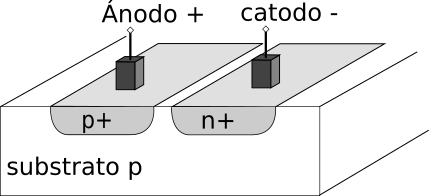
\includegraphics[width=0.4\textwidth]{img/diodo.png}
	\caption{Estructura física de un diodo de unión PN}
	\label{fig:diodo}
\end{figure}

\subsection{Transistores bipolares}\label{cap:bipolares}
\paragraph{}
También se pueden crear transistores de unión bipolar a partir de la creación
de dos uniones PN enfrentadas. En el caso de tener substrato P podemos conseguir
de forma sencilla un transistor tipo \textbf{PNP}, creando un contacto al substrato
P para el Colector (C), un pozo N dónde se crea un contacto a N+ para la base (B), y
una difusión positiva P+ dentro del pozo N, que funcionará como emisor (E).
Véase la figura \ref{fig:pnp}:

\begin{figure}[h]
	\centering
	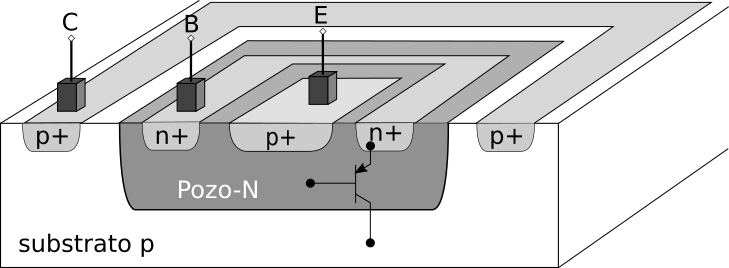
\includegraphics[width=0.7\textwidth]{img/pnp.png}
	\caption{Estructura física de un transistor de unión bipolar PNP}
	\label{fig:pnp}
\end{figure}

\paragraph{}
Crear un transistor NPN en una tecnología de substrato P es algo más complicado,
pero afortunadamente, existe la posibilidad de crear una estructura especial, que
va a ser muy usada en algunos casos con diferentes finalidades. Se trata del
llamado \textit{pozo N profundo} (\textit{Deep-N-Well} en inglés), que no
es más que un pozo N enterrado baja una capa de substrato P, que queda aislada del
substrato P del resto del chip si las uniones PN que forma con ambos substratos P,
están polarizadas inversamente.

\paragraph{}
De ésta forma podemos crear un transistor NPN entre el substrato profundo N,
colector (C), el substrato P encerrado por el anterior, base (B), y una difusión
N+ en el centro de este substrato P, que funcionará como emisor (E). Véase la
figura \ref{fig:npn}:

\begin{figure}[h]
	\centering
	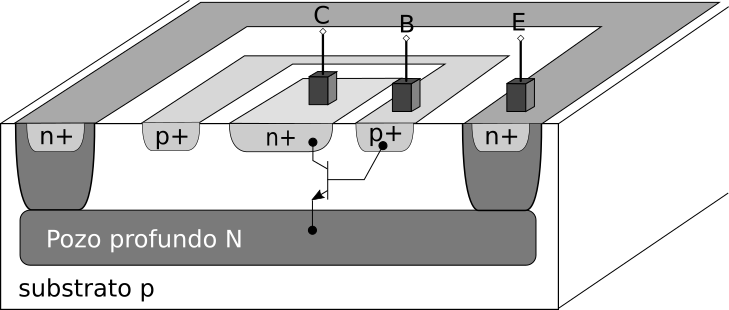
\includegraphics[width=0.7\textwidth]{img/npn.png}
	\caption{Estructura física de un transistor de unión bipolar NPN}
	\label{fig:npn}
\end{figure}

%WARNING
%Aniadir si es posible algun otro dispositivo en tecnologia CMOS

\section{Diseño de layout}\label{cap:layout}

\paragraph{}
El término \textit{layout} hace referencia a la implementación física del circuito
electrónico que se quiere fabricar. El layout consiste en un dibujo con toda
la información que necesita la empresa fabricante para implementar el circuito
sobre la oblea de silicio. Dicha información se representa por medio de "capas"
que se distribuyen en un espacio bidimensional. Cada capa tiene un significado y
unas normas que cumplir. El trabajo del diseñador de layout es definir, dibujar y
verificar el layout de los diferentes bloques que componen el chip siguiendo
las normas dadas por el fabricante, y procurando el mejor funcionamiento posible
del circuito en el menor area que le sea posible.

Como veremos más adelante, el diseño del layout de un circuito afecta o puede afectar
mucho al funcionamiento final del mismo.

\subsection{Capas de layout}\label{cap:capas_layout}

\paragraph{}
Todo diseño de layout está compuesto de una cierta cantidad de capas, de las cuales
algunas tienen significado físico directo y otras son capas que usa el software de
diseño para verificaciones o para cambiar propiedades de otras capas.

\paragraph{}
Naturalmente, los nombres de estas capas están asignados por cada fabricante en
concreto, pero los nombres que presento aquí para describirlas son los que usaré
para identificarlas durante el resto del documento.

\paragraph{NWELL}
Esta capa define el pozo N en una tecnología de substrato P. En ella se deben
situar los transistores PMOS y normalmente se polariza mediante difusiones \textbf{P+}
a la tensión más alta del circuito (VDD o similar).

\paragraph{WB}
Esta capa define el pozo enterrado (del inglés \textit{Well Buried}), o también
llamado pozo profundo (\textit{Deep-N-Well}), y como se introdujo en el capítulo
\ref{cap:bipolares}, donde se usaba para crear transistores bipolares. Esta
estructura también puede ser usada para crear zonas de substrato P aisladas del substrato
P del resto del chip. Dentro de esta zona se pueden disponer, por ejemplo, circuitos
CMOS digitales, con objeto de aislar el ruido que puedan generar a circuitos analógicos
cercanos.

\paragraph{XN}
Zona de difusión con dopado negativo N+, estará en las difusiones de drenador/fuente
de los transistores NMOS y en los contactos a substrato de los pozos N.

\paragraph{XP}
Zona de difusión con dopado positivo P+, de manera complementaria a la XN,
se usará para las difusiones de drenador/fuente
de los transistores PMOS y para los contactos al substrato P.

\paragraph{ACTIVE}
La capa activa indica al fabricante las zonas en las que se debe eliminar el óxido grueso (óxido
de campo). Ésto lo haremos siempre que haya que contactar una zona de difusión N o P,
o queramos crear la puerta de un transistor como se explica en el siguiente párrafo.

\paragraph{GC}
Zona donde se creará una capa de polisilicio o (\textit{poly}). Si coincide con capa activa,
se crearán puertas de transistores sobre una fina capa de óxido de silicio,
al cual llamaremos \textit{óxido de puerta}.
En los lugares donde no coincida con area activa se construirá sobre oxido grueso,
de espesor no tan controlado, y se usará para rutar líneas o para crear resistencias
de poly.

\paragraph{CS}
Contacto. Normalmente son cuadrados que definen contactos entre el Metal 1 y el
polisilicio (si están, respectivamente, sobre M1 ó GC), o al substrato, teniendo que
usar la capa ACTIVE para poder bajar al substrato.

\paragraph{M1}
Metal 1. Es el primero de los metales y se suele usar para contactar
transistores entre sí y con otros dispositivos, o para crear anillos de contactos
a substrato.

\paragraph{M2-M3-...-(M5)}
Otros metales. En función de la tecnología, pueden ser
más o menos capas de metal, por ejemplo 4 ó 6. La última capa de metal puede ser
diferente, ser más gruesa y menos resistiva, con objeto de usarse como caminos de
alimentación, que deben soportar corrientes mayores. Habitualmente, para seguir un órden
y ayudar al rutado del circuito, se suele definir un criterio de direcciones
en función de si la capa de metal es par o impar se dispondrán verticales u
horizontales. Mientras no se diga lo contrario, en el texto se usará el criterio
horizontal = impar, vertical = par.

\paragraph{V2-V3-...-(V5)}
Vías. Crean conexiones verticales entre un metal y el
inmediato superior. Se suelen usar varios para cada conexión por evitar una
posible rotura y para disminuir la resistencia total.

\paragraph{SA}
Del vocablo inglés \textbf{salicide}, que es una contracción de "\textbf{s}elf-\textbf{a}ligned si\textbf{licide}",
ésto es, siliciuro auto-alineado. Siliciuro es cualquier compuesto binario de
Silicio con otro elemento, generalmente metal; por ejemplo: CoSi\textsubscript{2}
ó TiSi\textsubscript{2}. Este siliciuro se dice auto-alineado porque el metal que
se deposita sobre el chip durante el proceso de fabricación se adhiere sólo sobre
dónde hay silicio (o poly), y no donde ya se ha hecho crecer la capa de óxido.
La reacción del silicio con el metal crea el siliciuro, lo que crea una capa más
conductiva que el silicio puro \cite{Maex:silicides}.

\paragraph{}
Por defecto todos el poly y las difusiones van silicidadas, pero usando la capa \textbf{SA},
podemos indicar que no se deposite siliciuro sobre algunas zonas, para, por ejemplo,
permitir que las resistencias de poly sean más resistivas.

\subsection{Herramientas de CAD}

\paragraph{}
Las herramientas de CAD (\textit{Computer Assisted Design}) se usan
en muchos campos de la ingeniería o la arquitectura, y actualmente, debido a la alta
complejidad de los diseños son de uso prácticamente obligado.

\paragraph{}
En el caso que nos ocupa, el diseño de circuitos microelectrónicos,
tiene gran importancia el buen uso y conocimiento de las herramientas por parte de
diseñadores. En nuestro caso, estas técnicas tienen dos finalidades fundamentales:
el diseño y simulación eléctrica y, por otro lado, la implementación física. Entre ellas
hay muchas diferencias, pero también existe una inevitable relación de dependencia.
La implementación física viene definida por el diseño eléctrico, pero a su vez, como
veremos en muchos casos, éste último condiciona el diseño eléctrico.

\paragraph{}
Por otra parte, en microelectrónica, debemos tener presente que
hay una división importante entre dos ámbitos que son bastante diferentes en cuanto
al flujo de diseño, simulación e implementación física, aunque ambos se basan sobre
la misma tecnología. Me refiero a la separación entre el ámbito \textbf{analógico}
y el \textbf{digital}. En éste trabajo nos centraremos en la parte analógica
puesto que el canal de lectura es un bloque fundamentalmente analógico.

\paragraph{}
Considerando únicamente el layout, estos dos ámbitos, analógico y
digital son también bastante diferentes. En el caso del layout digital, el flujo
de trabajo, debido a la gran cantidad de dispositivos que habitualmente son necesarios
para diseñar cualquier bloque digital, está altamente automatizado por algoritmos
de distribución y rutado automático (\textit{place and route}). Mediante estas
herramientas, el diseñador digital de back-end implementa el layout de un bloque
digital que el diseñador de front-end ha diseñado para que tenga un funcionamiento
definido.

\paragraph{}
Las herramientas de \textit{place and route} consisten en algorítmos
de posicionamiento de los sub-bloques digitales que conforman un macro-bloque:
inversores, buffers, puertas lógicas, flip-flops... La herramienta, considerando el
rutado entre cada bloque, los posiciona y los interconecta de forma que los tiempos
de propagación de las señales entre ellos estén dentro de unos márgenes aceptables.
En ocasiones, esta implementación física da problemas por cuestiones de congestión
de rutado, o por problemas de \textit{timing}, las señales no se propagan con la
suficiente velocidad y ésto genera fallos en el funcionamiento general de bloque.
Por todo esto, es muy importante la simulación post-layout de los bloques digitales.
Éstas tienen en cuenta los tiempos de respuesta de los sub-bloques digitales, los cuales
han sido obtenidos previamente mediante simulaciones analógicas, o vienen dados por
el fabricante de la tecnología en unos ficheros que incluyen tiempos y capacidades de
sus nodos. Posteriormente la herramienta considera las capacidades de las líneas de
rutado entre los sub-bloques, mediante un extraído de parásitos. Con todo ésto
se obtiene una simulación bastante cercana al comportamiento real del bloque una vez
fabricado, aunque nunca se puede asegurar al cien por cien el correcto funcionamiento
de todo el chip, lo que genera chips defectuosos en cada oblea fabricada.


\paragraph{}
Para el caso analógico, el editor de layout consiste en un software
de diseño gráfico en 2 dimensiones, dónde el diseñador de layout va dibujando los
dispositivos, y los va interconectando mediante líneas de rutado en los diferentes
metales que tiene a su disposición. El proceso es mucho más manual que en el caso
digital, dada la relativa simplicidad de los circuitos analógicos, frente a los
digitales. Un bloque analógico es abordable por una persona en unos pocos días o
semanas, ayudándose obviamente, de herramientas de replicación, jerarquizado, celdas
prediseñadas o parametrizadas. El caso analógico también se realiza de forma más
manual debido a la naturaleza de las señales analógicas, al ser éstas, en algunos casos,
más susceptibles a ruidos ,interferencias o acoplos con otras señales.

\paragraph{}
En los circuitos puramente digitales, las señales cambian de un
valor alto (1) a un valor bajo (0), siendo menos importante el valor exácto
mientras éste se encuentre dentro de los márgenes definidos. Por el contrario,
en un circuito analógico, hay que tomar cuidado en diseñar un layout que preserve
los valores de las señales anlógicas y tenga un impacto mínimo en los tiempos de
propagación o asegurar que dos dispositivos o bloques que deban comportarse idénticamente
así lo hagan.

\subsection{Problemas habituales en el diseño de layout}

\paragraph{}
A continuación se van a exponer y explicar algunos de los problemas habituales que
afectan a cualquier diseño de layout y que el diseñador debe hacer frente para
resolver o minimizar mediante su experiencia y la ayuda de las herramientas, de CAD,
la simulación post-layout y los consejos del diseñador analógico del bloque en cuestión.

\subsubsection{Area}

\paragraph{}
La superficie sobre la que se diseña un chip es limitada, y además es
un factor en contra del beneficio económico que tendrá la fabricación y venta del
chip. A menor sea el area usada por el chip, más chips caben en cada oblea, que tiene
un precio constante, definido por el fabricante en función de la tecnología y otros
parámetros. Por lo tanto, como punto de partida, podemos concluir que \textbf{el área
es siempre un parámetro a minimizar}, a cualquier nivel de jerarquía.

\paragraph{}
Si bien esto es la idea general, también es verdad que no siempre es
la prioridad, o bien el área no supone un problema porque, por ejemplo, debido a la
distribución de los bloques, un bloque resulte disponer de area más que suficiente.
Puede darse el caso incluso de que se prefiera distribuir un circuito de manera más
holgada pero más uniforme, antes que arrinconar todo el circuito en una zona y dejar
espacio libre en otras zonas. Ésto, por ejemplo, podría ayudar a mejorar la correlación
entre dispositivos, o \textit{matching}.

\subsubsection{Mismatch}

\paragraph{}
El mismatch es un problema generalizado en muchos campos de
la ingeniería donde se requiere la construcción de dispositivos que se comporten
igual, y por problemas de fabricación u otros agentes externos se comportan ligeramente
diferente.

\paragraph{}
En el caso del layout el mismatch puede deberse al proceso de fabricación,
que puede crear dispositivos de \textbf{dimensiones ligeramente mayores o menores},
o otorgar al silicio propiedades ligeramente diferentes, como la \textbf{concentración de
dopado}, lo que puede hacer que unas zonas sean mas o menos conductivas o que varíen
parmámetros como la tensión umbral.

\paragraph{}
Otra forma de que se creen diferencias entre unos dispositivos y otros
independientemente de la fabricación, es por ejemplo por la \textbf{distribución irregular
de la temperatura} cuando el chip esté funcionando. Debido a la ley de Joule, cualquier
corriente circulando por un material, lo calentará en función de la densidad de corriente
que lo atraviese. Si en una zona del chip tenemos un bus de alimentación, o un circuito
que consuma mucha corriente, calentará la zona cercana, creando gradientes de temperatura.
Si tenemos dos circuitos o dispositivos, uno de ellos cerca y otro lejos de esta zona,
posiblemente no se comporten igual.

\paragraph{}
Para minimizar los efectos de los gradientes, se suelen usar estructuras
de centroide común, que en teoría, para gradientes lineales, logran el emparejamiento
perfecto. Por ejemplo, si tenemos un array lineal de dos tipos de dispositivos diferentes,
cada uno con una multiplicidad de 4, deberíamos usar una estructura ABBA$\vert $ABBA, en vez
de AAAA$\vert $BBBB, dónde A y B representan instancias del mismo dispositivo. En el primero
de los casos, si existe un gradiente lineal en la dirección del array, el efecto de éste
actuará en positivo en unos y en negativo en otros, de forma que el efecto en A se compensa
al efecto en B. En cambio en el segundo caso, como promedio, los A sufrirán el efecto
más o menos que los B.

\paragraph{}
Ésto se puede aplicar también para arrays bidimensionales de dispositivos,
de forma que se pueden usar estructuras como la que se muestra en la figura \ref{fig:centroide_comun}:

\begin{figure}[h]
	\centering
	\includesvg[width=0.7\textwidth]{svg/common_centroid.svg}
	\caption{Estructura de centroide común}
	\label{fig:centroide_comun}
\end{figure}

\paragraph{}
Algunas de las reglas que se recomienda seguir para un buen matching entre transistores
serían \cite{Hastings2001:mos_matching}:

\begin{enumerate}
	\item Usar dimensiones idénticas para los \textit{fingers} del transistor,
	esto es, cada uno de los transistores unitarios dispuestos en paralelo,
	que forman uno mayor.
	\item Maximizar el área ($L \times W$) de los transistores, ya que las
	variaciones relativas en tamaños son menores.
	\item Orientar los transistores en la misma dirección, ya que el silicio
	puede presentar alguna anisotropía inherente a la fabricación.
	\item Situar los transistores lo más cerca posible entre ellos. A mayores
	distancias, mayores pueden ser las diferencias de temperatura, dopado, ruido...
	\item Uso de estructuras de centroide común.
	\item A ser posible, uso \textit{dummies} en los contornos del
	array de transistores. Un transistor, o en general, dispositivo \textit{dummy},
	es idéntico a uno activo en cuanto a construcción física, pero conectado de
	forma que no actúa eléctricamente, por ejemplo, un transistor CMOS podría
	conectarse a tierra todos sus terminales.
	Con esto evitamos los posibles efectos de borde que afectan un dispositivo
	que no tiene menos vecinos que los del interior del array.
	\item Colocar los dispositivos lejos de dispositivos de potencia o lineas
	de alimentación que pueden generar fuertes gradientes de temperatura.
	\item Intentar no rutar metal sobre la zona activa de los transistores,
	aunque esto es en muchos casos inviable. En caso de tener que hacerlo, tratar
	distribuir el metal de la forma más simétrica posible, afectando a todos
	los dispositivos por igual.
\end{enumerate}

%WARNING
%Detallar estas buenas prácticas
